Esta seção tem como objetivo mostrar a metodogia para implementação do trabalho
proposto. Primeiramente é mostrada a forma sequencia de como foi implementado os
algoritmos. Logo em seguida é apresentada a proposta de paralelização das tarefas
sequenciais utilizando a metodologia PCAM.

\begin{subsection}{Forma Sequencial Implementada}
A Figura~\ref{fig:gray} mostra o fluxograma da forma sequencial das tarefas
implementadas neste trabalho. Cada algoritmo realiza a conversão em escala de
cinza de imagens contidas em uma base com 5 mil imagens que são processadas um
por vez por cada algoritmo seguindo uma ordem sequencial de cada algoritmo
aplicado.  

\begin{figure}[!h]
	\centering
	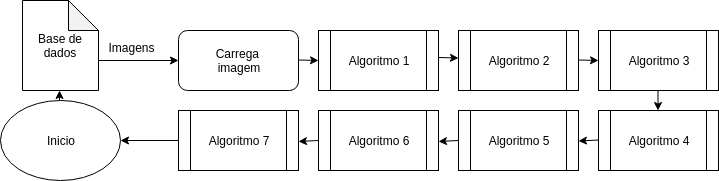
\includegraphics[width=0.95\linewidth]{figs/Sequential.png}
	\caption{Forma sequencial do algoritmo.}
	\label{fig:gray}
\end{figure}



A maioria das imagens digitais é composta por três canais de cores separados: um
canal vermelho, um canal verde e um canal azul. A sobreposição desses canais em
camadas cria uma imagem colorida. Modelos de cores diferentes têm canais
diferentes (às vezes os canais são cores, às vezes são outros valores como
luminosidade ou saturação), mas este trabalho se concentra apenas no RGB.

Todos os algoritmos de conversão do canal RGB para escala de cinza utilizam 
o mesmo processo básico que consistem em três etapas:

\begin{itemize}
\item Obter os valores dos canais vermelho, verde e azul de um \textit{pixel}.
\item Relacionar esses valores para transformar em apenas um valor.
\item Substituir os valores originais de vermelho, verde e azul pelo valor calculado
\end{itemize}


\begin{lstlisting}
for each pixel na imagem{

	vermelho = pixel.Red()
	verde = pixel.Green()
	azul = pizel.Blue()

	Obter_Valor_Cinza = cinza

	pixel.Red = cinza
	pixel.Green = cinza
	pixel.Blue = cinza

}
\end{lstlisting}


A Figura~\ref{fig:example} mostra o resultado da conversão em escala de cinza
para cada algortimo utilizado neste trabalho.  Os métodos para obtenção do valor
cinza para cada algorimo são apresentados a seguir.

\begin{figure}[!h]
	\centering
	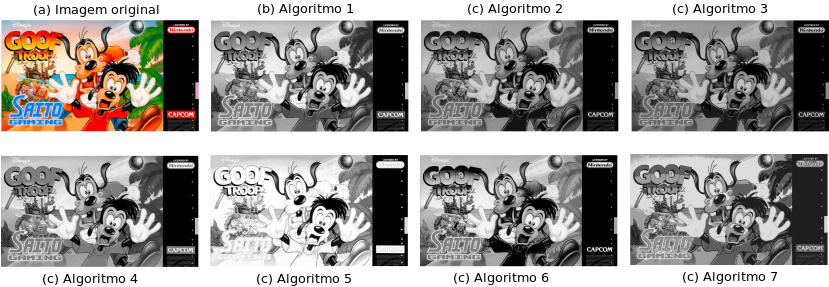
\includegraphics[width=0.95\linewidth]{figs/gray.png}
	\caption{Resultado dos algoritmos.}
	\label{fig:example}
\end{figure}

\subsubsection{Algoritmo 1: Média}
O algoritmo baseado na média é a rotina de conversão mais comum em escala de
cinza e o calculo do valor de cinza é obtido a partir da Equação~\ref{eq:media}.

\begin{equation}
\label{eq:media}
cinza = (vermelho + verde + azul)/3
\end{equation}

Essa fórmula gera um equivalente em escala de cinza razoavelmente boa e sua
simplicidade facilita a implementação e otimização. No entanto, esse método não
deixa de ter falhas --- embora rápida e simples, ela faz um mau trabalho em
representar tons de cinza em relação à maneira como os seres humanos percebem a
luminosidade (brilho).


\subsubsection{Algoritmo 2: Luminância}
Esse segundo algoritmo mostra que a densidade do cone no olho humano não é
uniforme entre as cores. Os seres humanos percebem o verde mais fortemente que o
vermelho e o vermelho mais fortemente que o azul. Isso faz sentido do ponto de
vista da biologia evolucionária --- grande parte do mundo natural aparece em
tons de verde, de modo que os humanos desenvolveram maior sensibilidade à luz
verde.

Como os humanos não percebem todas as cores da mesma forma, o ``método da média'' de
conversão em escala de cinza é impreciso. Em vez de tratar as luzes vermelha,
verde e azul igualmente, uma boa conversão em escala de cinza pondera cada cor
com base na maneira como o olho humano a percebe. Uma fórmula comum em
processadores de imagem (Photoshop, GIMP) é apresentada na
Equação~\ref{eq:luminancia}.


\begin{equation}
\label{eq:luminancia}
cinza = (0.3*vermelho + 0.59*verde + 0.11*azul)
\end{equation}

\subsubsection{Algoritmo 3: Luma}

Assim como no algoritmo 2, este método tenta uniformizar a forma como o ser
humano perceber as cores. Para isso, também é utilizada uma média ponderada
entre os canais como é mostrado na Equação~\ref{eq:luma}

\begin{equation}
\label{eq:luma}
cinza = (0.2126*vermelho + 0.7152*verde + 0.0722*azul)
\end{equation}


\subsubsection{Algoritmo 4: Dessaturação}

A maioria dos programadores usa o modelo de cores RGB. Embora seja uma boa
maneira de uma máquina descrever cores, o espaço de cores RGB pode ser difícil
para a percepção humana. Nesse sentido, o espaço de color HSL (do inglês
\textit{hue, saturation, lightness}) é algumas vezes utilizado para a
vizualização das cores. A matiz (\textit{Hue}) pode ser considerada o nome da
cor --- vermelho, verde, laranja, amarelo etc.  A saturação
(\textit{saturation}) descreve como uma cor é vívida; uma cor muito vívida tem
saturação total, enquanto o cinza não tem saturação. 

A dessaturação de uma imagem funciona convertendo o espaço RGB no espaço HSL e 
forçando a saturação para zero. Um pixel pode ser dessaturado encontrando o
ponto médio entre o máximo de (R, G, B) e o mínimo de (R, G, B), como mostra a
Equação~\ref{eq:dessatura}.

\begin{equation}
\label{eq:dessatura}
cinza = ( Max(vermelho, verde, azul) + Min(vermelho, verde, azul) ) / 2
\end{equation}



\subsubsection{Algoritmo 5: Decomposição}
A decomposição de uma imagem oPde ser considerada uma forma mais simples de
dessaturação. Para decompor uma imagem, cada \textit{pixel} é forçado parao
valor mais alto (máximo) ou mais baixo (mínimo) de seus valores em vermelho,
verde e azul. As Equações~\ref{eq:a} e~\ref{eq:b} mostram como calcular a
decomposição máxima e mínima, respectivamente.

\begin{subequations}

\begin{equation}
\label{eq:a}
cinza = Max(vermelho, verde, azul) 
\end{equation}

\vspace{-1cm}

\begin{equation}
\label{eq:b}
cinza =  Min(vermelho, verde, azul) 
\end{equation}
\end{subequations}


\subsubsection{Algoritmo 6: Canal de cor única}

Este algoritmo representa o método computacional mais simples para conversão em
escala de cinza. Ao contrário de todos os métodos apresentados, este método 
não requer cálculos. Apenas é necessário escolher o valor de um determinado
canal e aplicar para ao valor de cinza, como mostrado na
Equação~\ref{eq:a1},~\ref{eq:b1} e~\ref{eq:c1}

\begin{subequations}

\begin{equation}
\label{eq:a1}
cinza = vermelho 
\end{equation}

\vspace{-1cm}

\begin{equation}
\label{eq:b1}
cinza =  verde 
\end{equation}

\vspace{-1cm}

\begin{equation}
\label{eq:c1}
cinza =  azul 
\end{equation}
\end{subequations}
  
\subsubsection{Algoritmo 7: Tons de cinza}
Este método permite ao usuário especificar quantos tons de cinza a imagem
resultante utilizará. O algoritmo definir o número de tons de cinza da imagem
convertida. Esse método é um pouco mais trabalhoso se comparado com os demais
algoritmos apresentados. Os procedimentos do algoritmo é mostrado a seguir.


\begin{lstlisting}
for each pixel na imagem{
	fator = 255 / (TonsDeCinza - 1)
	metodo = (vermelho + verde + azul)/3
	cinza = (int)((medio / fator) + 0.5) * fator

	//TonsDeCinza: valor entre 2 e 256
}
\end{lstlisting}

\end{subsection}

\begin{subsection}{Projeto da Forma Paralela}
O projeto da forma paralela segue a metodologia PCAM (Particionamento,
Comunicação, Agrupamento e Mapeamento) descritra a seguir.

\begin{itemize}
\item \textbf{Particionamento}: Quebra do problema em subproblemas menores.
\item \textbf{Comunicação}:Definição da comunicação entre as várias tarefas que
foram subdivididas.
\item \textbf{Agrupamento}: Combinação das tarefas de forma a se estabelecer a
comunicação, se necessário, visando reduzir custos
\item \textbf{Mapeamento}: Escolha de quais tarefas vão ficar em cada processador.

\end{itemize}

\subsubsection{Particionamento}
Como o Raspberry Pi Modelo B utilizado para executar o programa desenvolvido
para teste trabalho possui 4 núcleos de processamento, é importante subdividir o
problema em subtarefas. Uma alternativa seria dividir os 7 algoritmos entre os
processadores. O problema desta abordagem é que um dos processadores ia executar
apenas um algoritmo, subutilizando-o em comparação aos demais núcleos. Outra
abordadem que pode ser utilizado, e a que provavelmente vai ser utilizada, é o
processamento de 4 imagens em paralel, onde cada núcleo seria encarregado de
executar os 7 algoritmos para suas respectivas imagens.

\subsubsection{Comunicação}

O programa desenvolvida a presenta 7 algoritmos de conversão em escala de cinza
de uma imagem e esses algoritmos são independentes entre si, o que torna a
implementação do paralelismo nessas tarefas sem a necessidade de realizar
comunicações entre os núcleos de processamento.

\subsubsection{Agrupamento}
Como não há a necessidade de comunicação entre as unidades de processamento,
cada núcleo será responsável por processar uma imagem, visto que se o particion
amento fosse projetado levando em consideração as tarefas, o agrupamento de
tarefas ficaria desbalanceado, subutilizando uma das unidades de processamento
(UP).

\subsubsection{Mapeamento}

O paralelismo vai ser aplicado na quantidade de imagens que devem ser
processadas e não na quantidade de algoritmos de conversão em escala de cinza.
Dessa forma, 4 imagens devem ser trabalhadas em paralelo, onde a primeira imagem
deve ser processada pela UP1, a segunda imagen pela UP2, a terceira imagem pela
UP3 e a quarta imagem pela UP4. Assim que as 4 imagens forem processadas, mais
4 novas imagens são dadas como entrada no sistema que refaz todo o processo.


\end{subsection}




